\section{Userverwaltung [L]}
\setauthor{Litzlbauer Lorenz}
Im Projekt wurde eine Userverwaltung eingebaut. Die User können sich auf der Weboberfläche anmelden und registrieren. Je nach Registrationsstatus (auf der Webseiten angemeldet oder nicht) stehen ihnen mehr Funktionalitäten zu Verfügung. Ein*e Besucher*in, die nicht angemeldet ist, kann alle Ausstellungen ansehen und auf der Suchunterseite nach Ausstellungen suchen. Ein*e registriert*er User*in könnte das auch, zusätzlich können sie auch ihre Profileseite sehen und Ausstellungen selbst erstellen und veröffentlichen. Die Navigationsleiste wurde so programmiert, dass sie dem*der User*in nur die Unterseiten zeigt, die diese durch ihrem Registrationsstatus auch besuchen kann. 

Im folgendem Abschnitt 'Sign-, Log-In Funktionalitäten' wird die Implementation des Userverwaltung und die damit verbundenen Features erklärt. 

\subsection{JWT - Json Web Token [L]}
Der Json Web Token (JWT) ist ein offenere Standard. Er wird durch RFC7519 definiert. JWT wird zur sicheren Übertragung von Informationen benutzt, indem er die Benützer authentifiziert. 

\paragraph{Struktur}
Der JWT besteht aus einem Header, einer Payload und der Signatur. 

\paragraph{Im Projekt}
Der JW





https://auth0.com/learn/json-web-tokens


\subsection{Implementation im Frontend [L]}
\setauthor{Litzlbauer Lorenz}
Nachdem der JWT im Backend implementiert wurde, galt es diesen auch auf dem Frontend einzubauen. Der JWT dient zur Authentifizierung des*der User*in und zum rollenbasierenden Schutz der API. 

\subsubsection{Sign- und Log-In}
Da der JWT als Beweis dafür dient, dass der*die User*in Authentifiziert ist, muss sich der*die Benutzer vor dem Erhalten des Token dafür erst auf der Weboberfläche Registrieren oder Anmelden. 

\begin{figure}
    \centering
    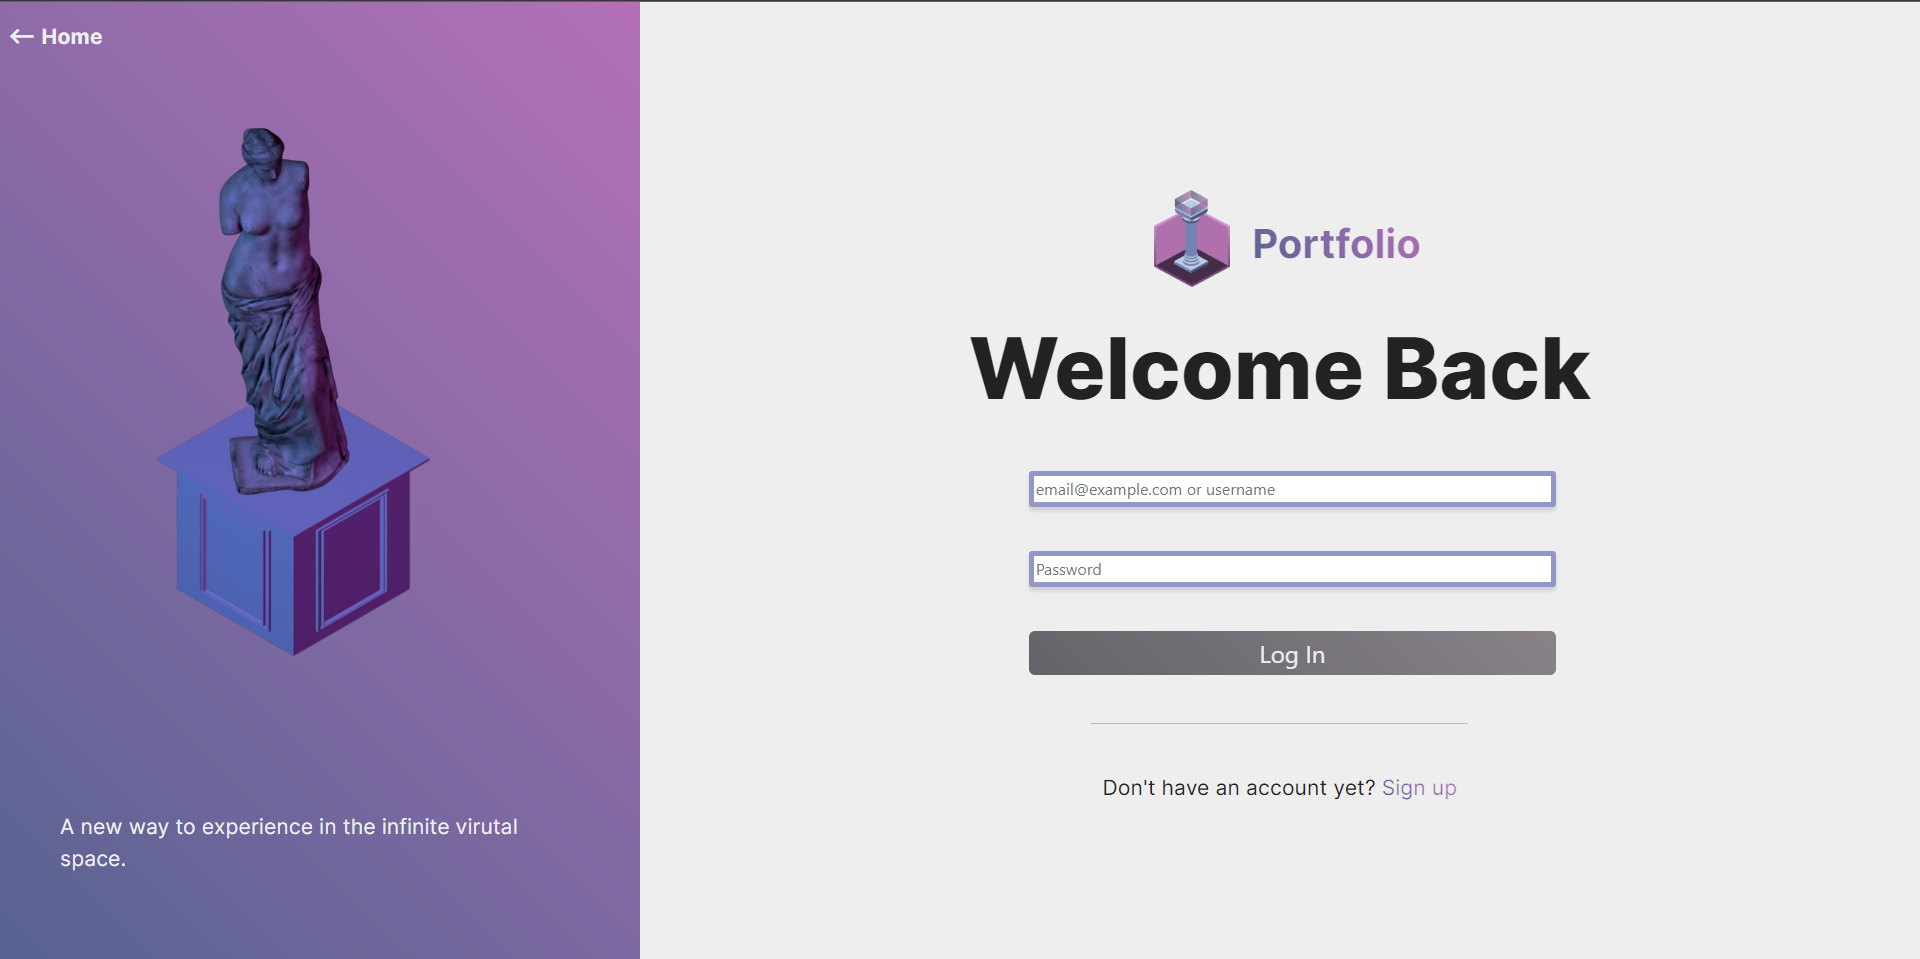
\includegraphics[scale=0.25]{pics/GalleryLogIn.png}
    \caption{Projekt: Login Page}
    \label{fig:impl:login}
\end{figure}

Für das Userinterface wurden Anmelde- und Registrierungs-Funktionalitäten implementiert (siehe Abbildung der Anmeldeseite \ref{fig:impl:login}). Die Anmelde- und Registrationsformulare wurden mithilfe von reaktiven Formularen und Validatoren (siehe Absatz \ref{par:impl:usermanagment:reactiveForms}) umgesetzt. Nachdem eine valide Eingabe von dem*der User*in gemacht wurde, aktiviert sich der Anmelde- bzw. Registrierungsknopf und lässt sich drücken. Die Aktivierung des Knopfes wird durch die Farbveränderung von Grau auf Bunt sichtbar gemacht.  Nachdem der*die User*in die Eingabe bestätigt hatte, indem sie*er den Knopf drückte, werden die Anmeldedaten über das HTTPS-Protokoll mithilfe des HTTP-Moduls (siehe Abschnitt TODO referzieren fabians http-module is not net commitet) an den Server gesendet. Nach einer erfolgreichen Anmeldung / Registration wird an die Weboberfläche eine Antwort geschickt, in der der JWT Token enthalten ist. Danach wird der*die User*in auf die Profilseite weitergeleitet. Bei einer gescheiterten Anmelde- / Registrierungsversuch wird der*die User*in durch eine Fehlermeldung darüber informiert.

Nach der erfolgreichen Anmeldung / Registration wird vom Server ein JWT ausgestellt. Bei einem HTTP-Request vom Client zum Server kann der JWT im Header des Requests platziert werden, der Server kann diesen auslesen und so feststellen, ob ein*e Benutzer*in auch wirklich authentifiziert ist.

Nun gibt es aber mehrere Unbequemlichkeiten, die aus diesem Prozess resultieren. Der*Die User*in muss sich jedes Mal, bei jedem neuen Webseitbesuch und beim neuen Laden der Webseite, neu anmelden und der*die Entwickler*innen müssen bei jedem HTTP-Request (also jeder Kommunikation mit dem Server) manuell den JWT in den Header platzieren.

\paragraph{Formulare und Validation}
\label{par:impl:usermanagment:reactiveForms}
In Webanwendungen gibt es viele Formulare, weil sie dort als eine der primären Kommunikationsschnittstellen zum Besucher*in dienen. Natürlich gibt es dafür den nativen Inputelement von HTML, aber zu einem Formular mit guter Usererfahrung gehört auch ein visuelles Feedback für den*die Benuzter*in, zusätzlich wächst der Entwicklungsaufwand exponentiell mit der Featureanzahl des Formulars.

Angular bietet verschiedene Implementierungsarten, um die visuelle Komponente umzusetzen und den Entwicklungsaufwand zu minimieren. Bei diesen Ansätzen können mehrere Eingabedaten zentral ausgewertet und weiterverarbeitet werden und der Status des Formulars bei Änderungen und Fehlern visuell dargestellt werden. \cite[Bookmonkey - 12 Formularverarbeitung und
Validierung: Iteration IV]{AngularBuch}

Bei den Ansätzen unterscheidet man zwischen den reactive Forms und den Template-Driven-Forms.

\subsubsection{Token-Verwaltung}
Um das Problem der Anmeldung zu lösen, wurde der JWT im LocalStorage des Browsers gespeichert. Im Codeausschnitt (siehe \ref{lst:impl:sign:jwtLocalstorage}) ist ein Teil des Authentifizierungsdienstes des Projektes zu sehen. Mit der Funktion \emph{setSaveJWT} wird der ausgestellte JWT ausgelesen und die darin enthaltenen Informationen, der Name und die Id des Benutzers, die Id des Tokens und das Ablaufdatum des Tokens im LokalenStorage (siehe im Absatz WebStorage API \ref{par:impl:usermanagment:WebStorage}) gespeichert, damit die Daten auch nach dem Neuladen der Webseite erhalten bleiben. Die Funktion \emph{isLoggedIn} gibt nach dem Aufruf den Status mit, ob eine Person angemeldet ist oder nicht, dafür benutzt die Funktion das im JWT enthaltene Ablaufdatum und vergleicht es mit dem aktuellen Datum. Zuletzt gibt es noch die \emph{logout} Funktion, diese löscht die im LocalStorage enthaltenen JWT-spezifischen Daten.

\begin{lstlisting}[caption=auth.service.ts - JWT und Localstorage,label=lst:impl:sign:jwtLocalstorage,language=TypeScript ]
export class AuthService {
    ...
    setSaveJWT(value: any) {
        let decodedJWTPayload = JSON.parse(atob(value.split('.')[1]))
        localStorage.setItem("user", decodedJWTPayload.sub)
        localStorage.setItem('id_token', value)
        localStorage.setItem('expires_at', decodedJWTPayload.exp)
        localStorage.setItem('user_id', decodedJWTPayload.userid)
      }

    isLoggedIn(): boolean {
        if (localStorage.getItem('id_token') && localStorage.getItem('expires_at')) {
          let temp = new Date().getTime()
          const exp = Number(localStorage.getItem('expires_at'))
          return temp < exp
        } else {
          return false;
        }
      }

    logout() {
        localStorage.removeItem("user")
        localStorage.removeItem('id_token')
        localStorage.removeItem('expires_at')
        localStorage.removeItem('user_id')
      }
    ...
}        
\end{lstlisting}

\paragraph{WebStorage API}
\label{par:impl:usermanagment:WebStorage}
Die WebSotrage API bietet verschiedene Möglichkeiten, Daten per Schlüssel-Werte-Paare im Web zu persistieren. Persistenz ist die Fähigkeit, Daten in einem nicht flüchtigen Speicher zu speichern, um so den Datenverlust beim Neustart des Systems zu verhindern. Die WebStorage API ist nicht Teil des DOM, sondern der globalen Web-Variable window. Die zwei Arten, Daten mittels der WebStorage API zu persistieren, sind der LocalStorage und der SessionStorage.
\cite{WikiPersistenzDefinition} \cite{WebStorageAPI}


\subparagraph{SessionStorage}
Daten im SessionStorage werden je nach ihrem Ursprung getrennt aufbewahrt. Sie werden für die Zeit der Webseitensession gespeichert, wenn der Browser oder der Tab geschlossen wird, sind die Informationen auch fort.
\cite{WebStorageAPI}

\subparagraph{LocalStorage}
Daten werden wie im SessionStorage auch persistiert, doch auch wenn der Browser geschlossen wird bleiben die Daten erhalten. Daten können nur durch JavaScript oder das Löschen des Webbrowser-Caches gelöscht werden.
\cite{WebStorageAPI}

\subparagraph{Allgemeine Informationen}
Beide Speichermethoden benutzen keine Server, um die Daten zu speichern, sondern den Cache des Webbrowsers. Das Speicherlimit hängt vom Webbrowser ab, doch beträgt es meistens 5 MB und es können nur Zeichenketten gespeichert werden.
\cite{WebStorageAPI}

\subsubsection{HTTP-Interceptoren}
HTTP-Interceptoren funktionieren in Angular als Zwischenschicht zwischen den ausgehenden HTTP-Abfragen und den eingehenden HTTP-Antworten und können diese umwandeln.
Das Einsatzgebiet von HTTP-Interceptoren ist bei globalen Änderungen und Funktionen, die an allen HTTP-Requests durchgeführt werden sollen. Es war somit das perfekte Werkzeug, um in allen HTTP-Requests den JWT in den Header zu verpacken.
\cite[10.3 Interceptoren: HTTP-Requests abfangen und transformieren]{AngularBuch}

Wenn ein Request an den Server geht, wird dieser unterbrochen. Es wird überprüft, ob der JWT verfügbar ist. Wenn das zutrifft, wird der ursprüngliche Request geklont, in der Authentifizierungsspalte des Headers wird die JWT-Id hinzugefügt, danach wird der Request wieder zum Server weitergeleitet (siehe Code \ref{lst:impl:sign:JWTInterceptor}). 

\begin{lstlisting}[caption=auth.interceptor.ts - add JWT to Request Header,label=lst:impl:sign:JWTInterceptor,language=TypeScript]
import { Injectable } from '@angular/core';
import {
  HttpRequest,
  HttpHandler,
  HttpEvent,
  HttpInterceptor
} from '@angular/common/http';
import { Observable } from 'rxjs';

@Injectable()
export class AuthInterceptor implements HttpInterceptor {

  constructor() {}

  intercept(request: HttpRequest<unknown>, next: HttpHandler): Observable<HttpEvent<unknown>> {

    const idToken = localStorage.getItem('id_token')
    if (idToken) {
      const cloned = request.clone(
        {
          headers: request.headers.set('Authorization', 'Bearer '.concat(idToken))
        }
      )

      return next.handle(cloned)
    }

    return next.handle(request);
  }
}
\end{lstlisting}

\subsubsection{Routing- und Navigations-Einschränkung}
Zum Start dieses Entwicklungsschrittes war der Interceptor und die JWT Verwaltung fertig. Doch das Projekt brauchte eine besseres visuelles Feedback System um dem*der Kunden*in zu den Anmeldestatus zu zeigen.

Deswegen und um zu verhindern das Benutzer*in auf Unterseiten sind auf denen sie wegen ihres Requistratonstatus (noch nicht authentifiziert) noch nichts machen können, wurde je nach Anmeldestatus andere Routen und Informationen auf der Navigationsbar gezeigt (siehe Abbildung \ref{fig:impl:navbarvergleich}). Dafür wurde die Navigationsleistenlogik und die Navigationsleistenservice angepasst. Zusätzlich wurde AuthGuard verwendet um Routen zu sperren auf, die der*die Benutzer*in wegen dem Requistratonstatus noch keinen Zugriff hat. 

\begin{figure}
  \centering
  \includegraphics[scale=0.5]{pics/navbarRequistrationsstatusGegenüberstellung.png}
  \caption{Navbar: authentifiziert vs noch nicht authentifiziert}
  \label{fig:impl:navbarvergleich}
\end{figure}


\subsection{Erledigte Userstories [L]}
Im Entwicklungsprozess des Usermanagment-System wurden folgende Userstories vollendet: 
\begin{compactenum}
  \item Als Designer möchte ich einen Login, um meine Ausstellungen speichern und im Nachhinein immer öffnen zu können.
  Akzeptanzkriterien:
  \begin{compactitem}
      \item Man kann sich neu registrieren
      \item Registrierung mittels Username und Passwort
      \item Das Passwort muss überprüft werden beim Erstellen und mind. 8 Zeichen enthalten
  \end{compactitem}
  \item Als User*in will ich andere Rechte haben, je nachdem ob ich angemeldet bin oder nicht. Auswahlkriterien:
  Wenn ein*e User*in angemeldet ist, kann er*sie:
      \begin{compactitem}
          \item Ausstellungen ansehen
          \item Ausstellungen erstellen/löschen
      \end{compactitem}  
  Wenn ein ein*e User*in nicht angemeldet ist, kann er*sie:
      \begin{compactitem}
          \item Ausstellungen ansehen
          \item keine Ausstellungen erstellen
          \item keine Ausstellungen favorisieren
      \end{compactitem} 
\end{compactenum}